\documentclass[a4paper,11pt]{article}
\usepackage{booktabs} % Provides professional-quality horizontal rules
\usepackage{float} % Required for [H] placement
\usepackage{tikz}
\usepackage{hyperref}
\usepackage{graphicx} 
% \graphicspath{ {./images/} } % Optional: Specifies the folder where your images are saved
% \usepackage[bottom=1.5in]{geometry} // push page footer down 
\setlength{\footskip}{100pt}
\usepackage[skip=4pt, font=tiny]{caption} 


\makeatletter
\renewcommand{\verbatim@font}{\tiny\ttfamily} % Changes to sans-serif
\makeatother


\hypersetup{
    colorlinks=true,    % True removes the default red/green border boxes
    linkcolor=blue,     % Colors internal links (like the TOC) blue
    urlcolor=cyan       % Colors external URLs cyan
}

\newcommand{\newpagex}{
    \newpage
    \vspace*{-7\baselineskip} % Pulls text up by one line
}

\author{Hectron} 

\title{Getting Started with App}

\begin{document}
    \maketitle
    \tableofcontents
    \newpagex
    \noindent

    \section{Description}
        Document informs the user how to start the application residing in the nba\_app  directory of repository ReactApps. 
        Applications were developed on MacOS \(Sonoma\). The following programming languages were used throughout fullstack development.
        \begin{itemize}
            \item \textbf{FrontEnd} \newline \textmd{Typescript - imperative}
            \item \textbf{Server}: \newline  \textmd{Typescript - imperative}
            \item \textbf{Backend}: \newline  \textmd{Postgres - declarative}
            \item \textbf{Script}: \newline  \textmd{Bash - imperative}
        \end{itemize}

    \section{Run Application}
        \begin{itemize}
            \item  Open Docker. If Docker is not installed, please download at \hypersetup{colorlinks=false,urlcolor=black } \url{https://www.docker.com/products/docker-desktop/} 
            \item Start/Configure Postgres Database (Docker Container Instance) 
            \begin{itemize}
                \item Change directory to nba\_app/database
                \item run run.sh 
            \end{itemize}
            \item Start Monitor Service.
                \newline 
            The highest priority service. All request are handled by the monitor service. The start monitor must be running for proper operation of the application. 
                \begin{itemize}
                \item Change directory to nba\_app
                \item run server/main.sh \quad \small \textit{Monitor service is now running }
            \end{itemize}

            \item Open web browser; request application at address and port \url{ http://127.0.0.1:50214/ }
        \end{itemize}
            

    \section{Figures}

        \noindent
        % O(nlog\_{2}(n)) search .This is a\_test. 
        \vspace*{-2\baselineskip} % Pulls text up by one line
        
        \begin{figure}[H]
            
            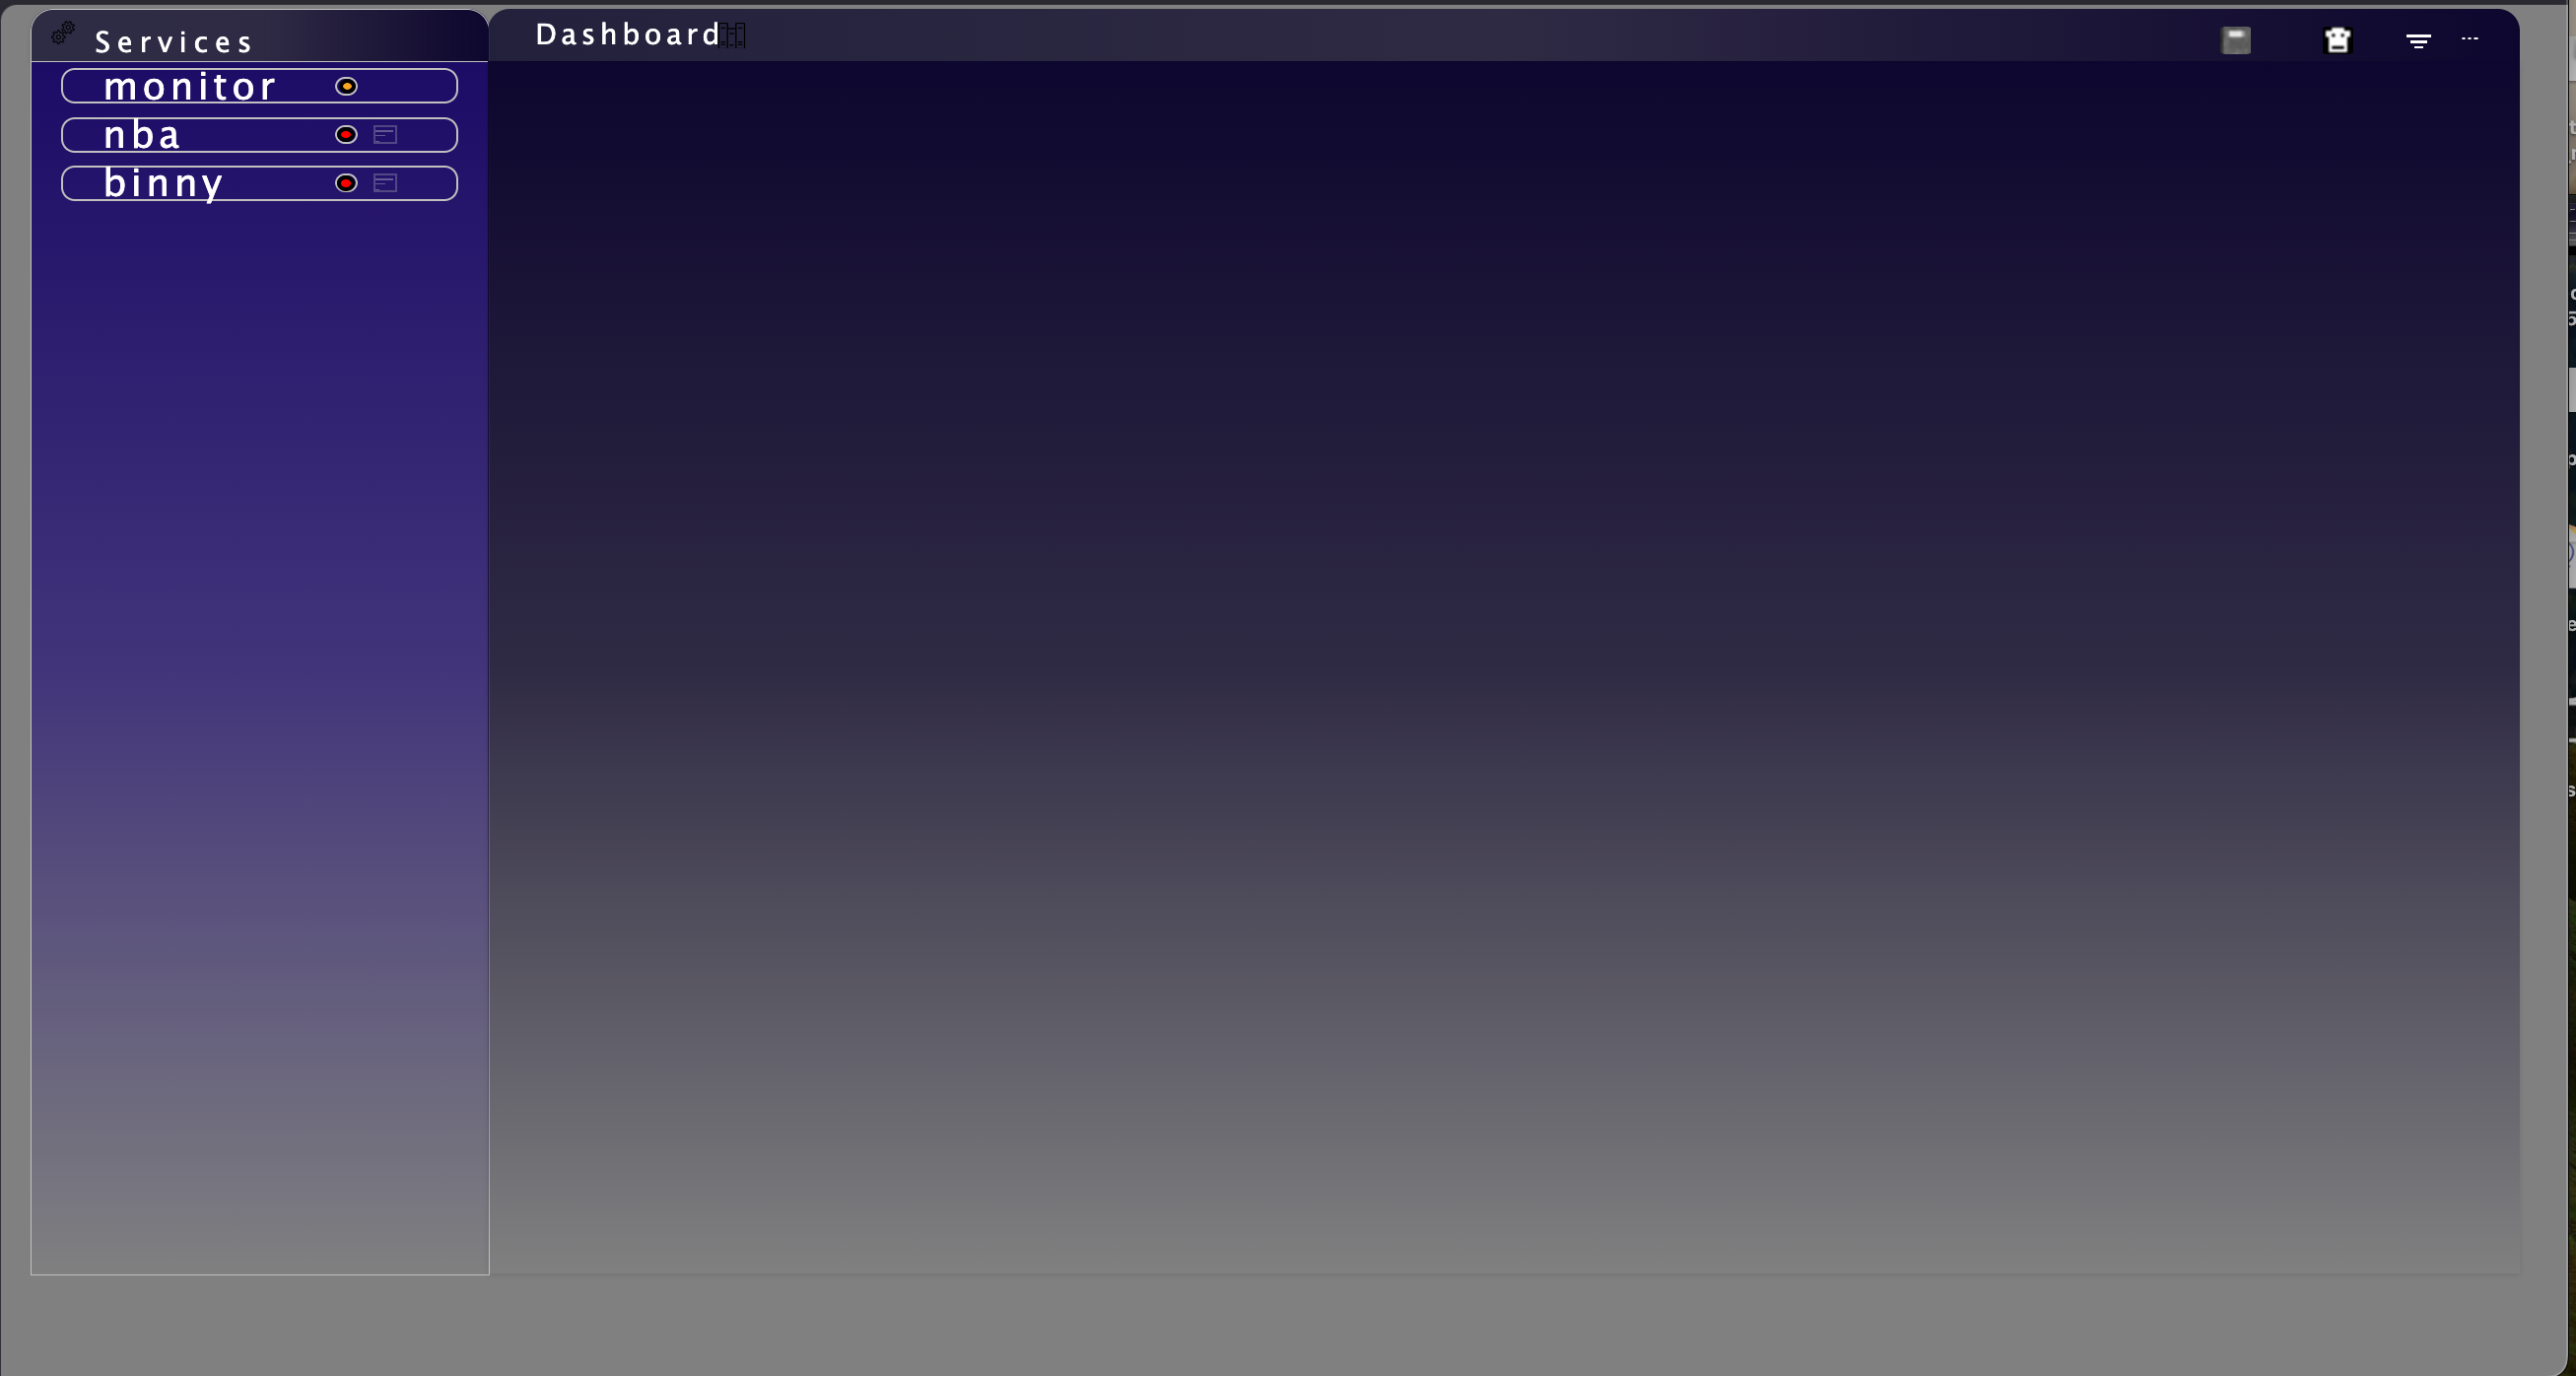
\includegraphics[width=1.0\textwidth, height=0.27\textheight]{image0}
            
            \caption{Home Page}
        
            \label{fig:home}

        \end{figure}
    
         \newpagex

        \begin{figure}[H]
            
            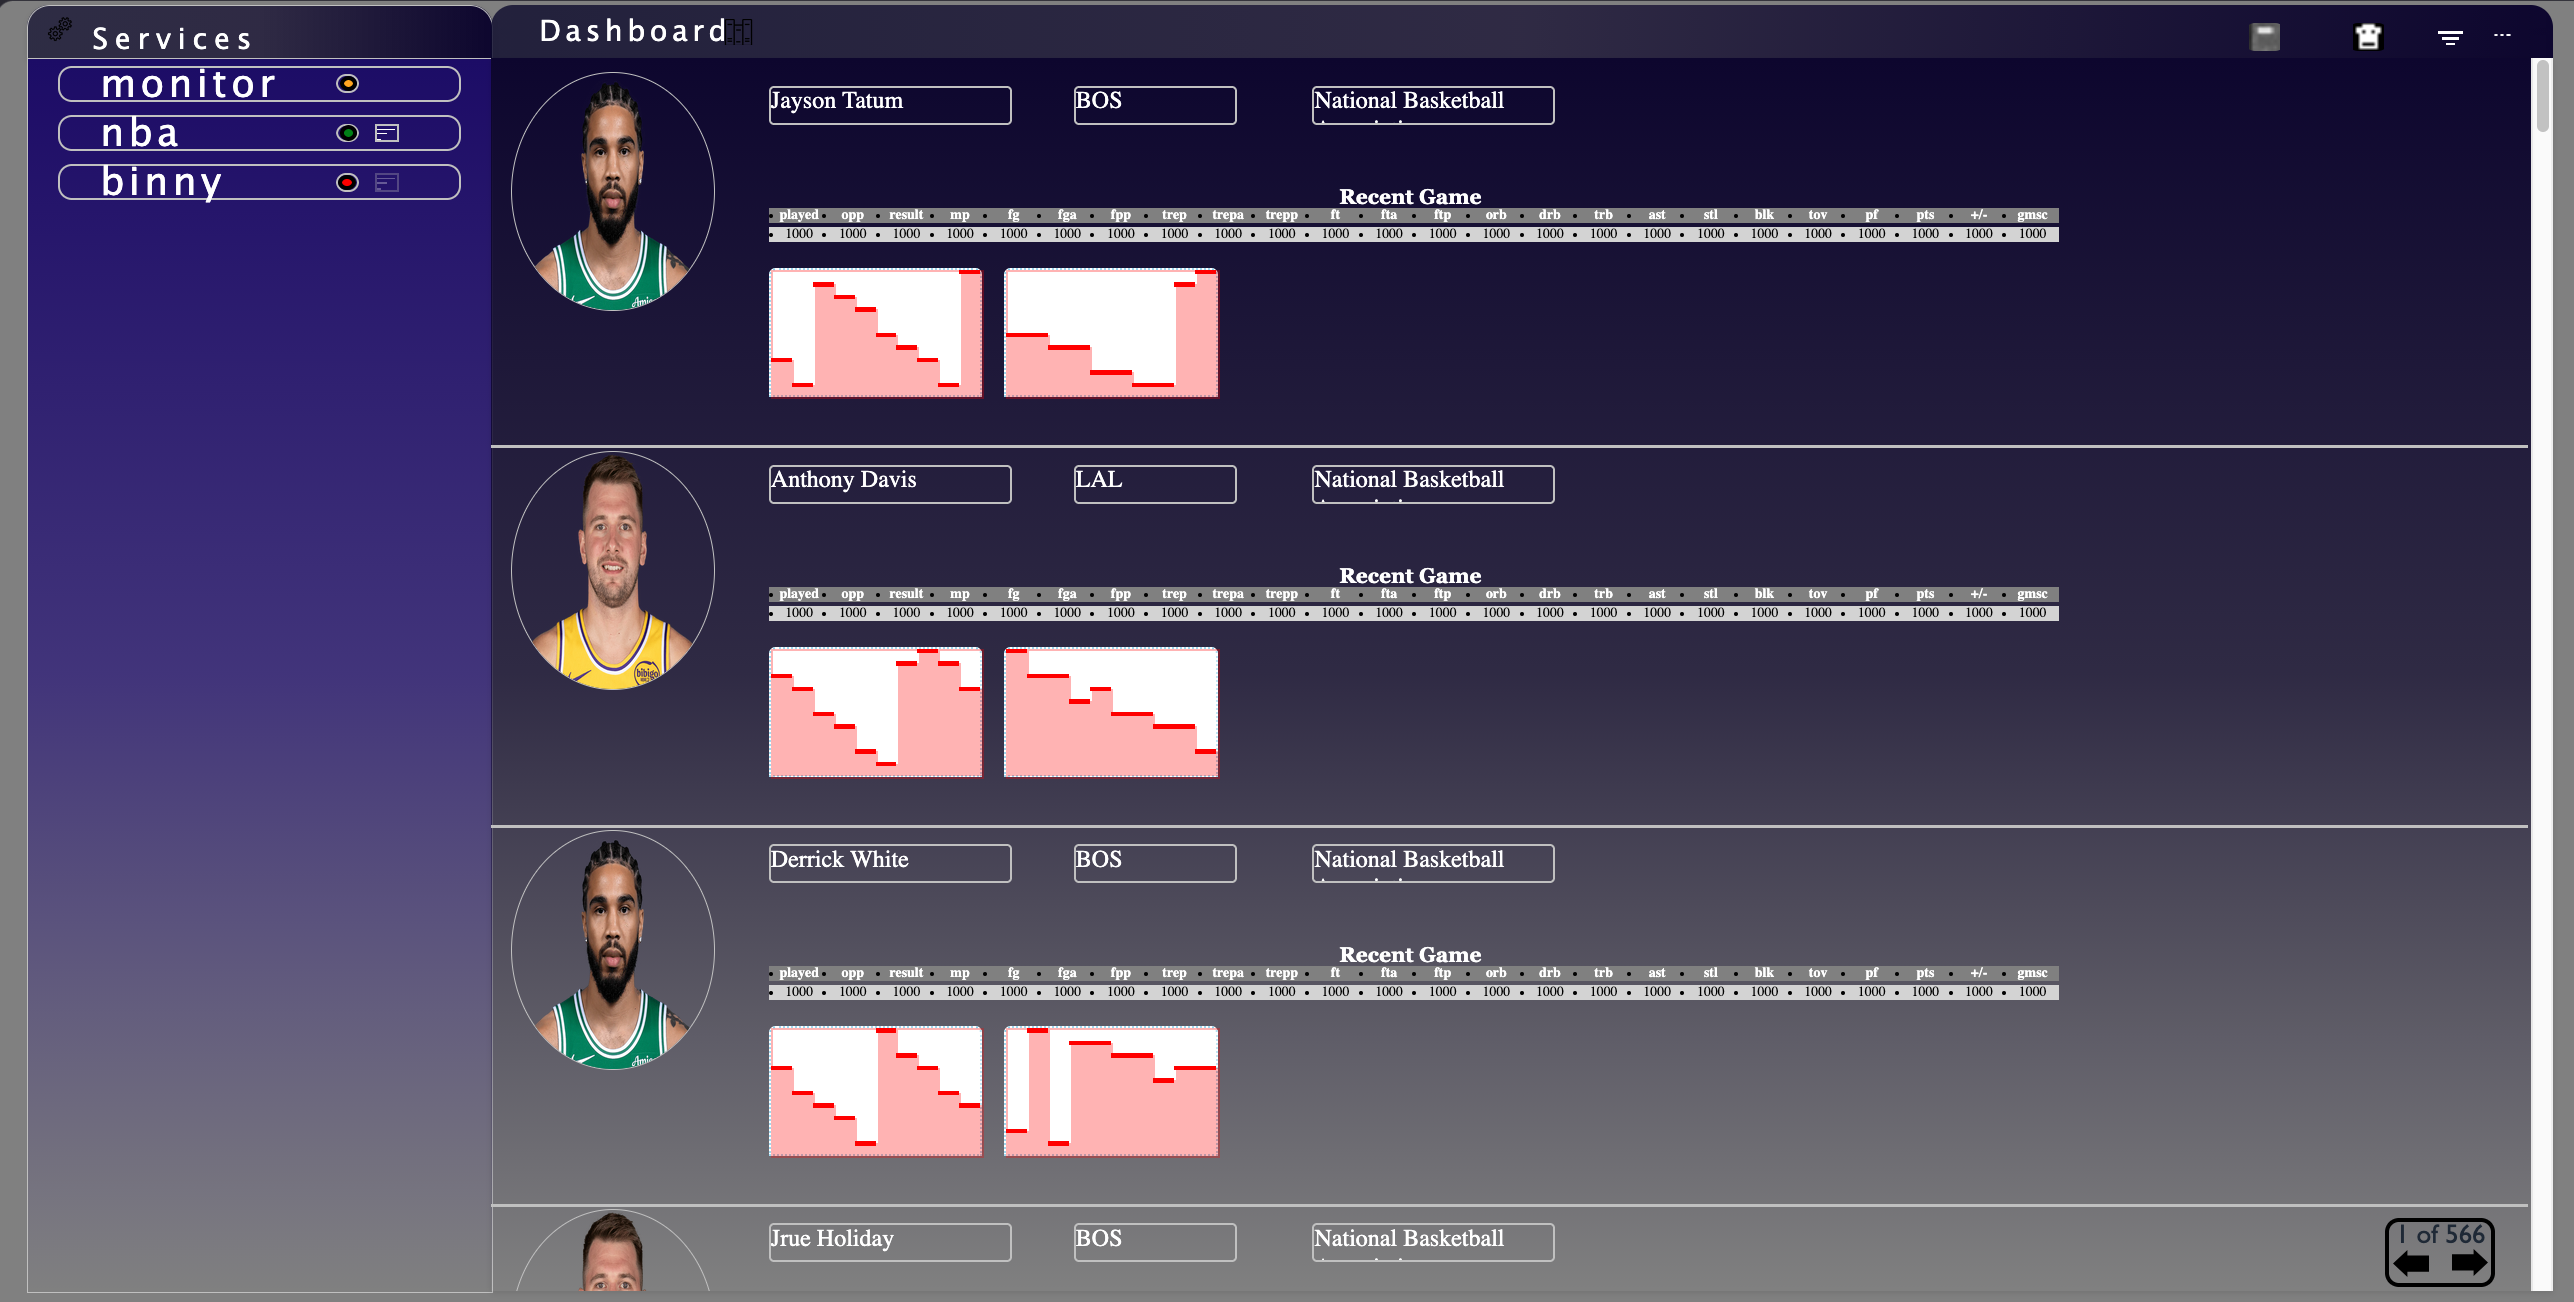
\includegraphics[width=1.0\textwidth, height=0.27\textheight]{image1}
            
            \caption{\textbf{GET} NBA Service}
        
            \label{fig:nba}

        \end{figure}

        \begin{figure}[H]
            
            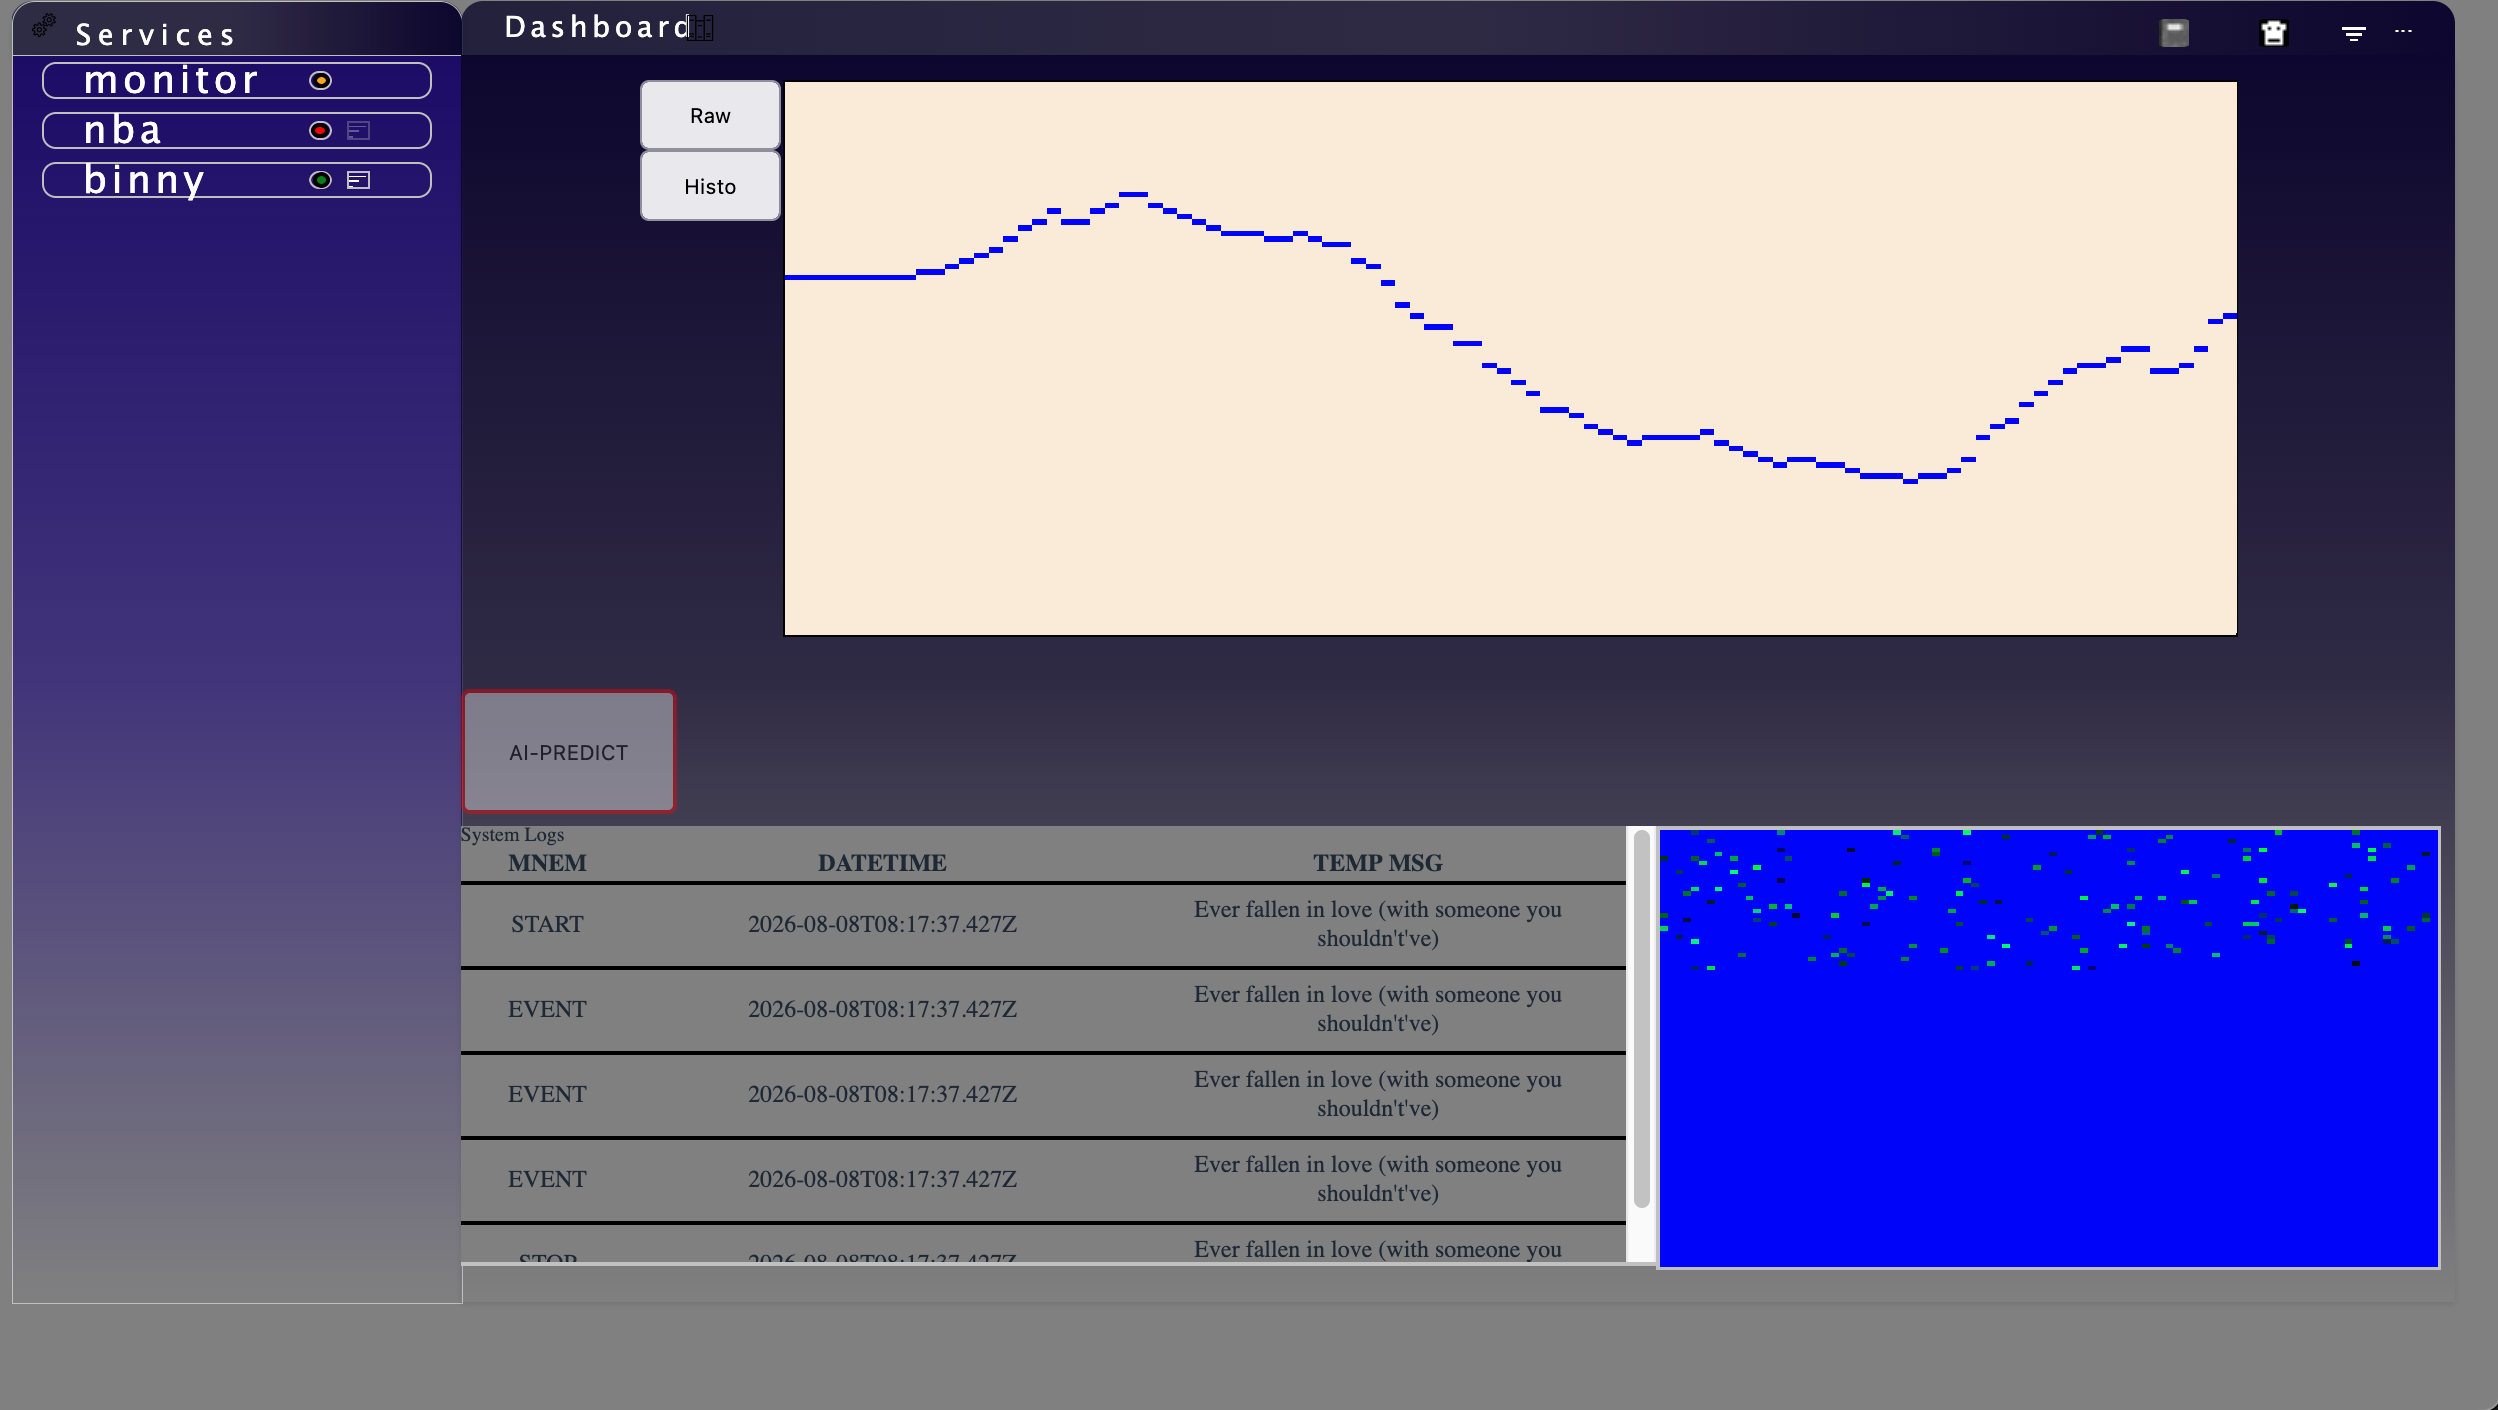
\includegraphics[width=1.0\textwidth, height=0.27\textheight]{image2}
            
            \caption{\textbf{GET} Binny Service - XY Plot}
        
            \label{fig:xybinny}

        \end{figure}

        \begin{figure}[H]
            
            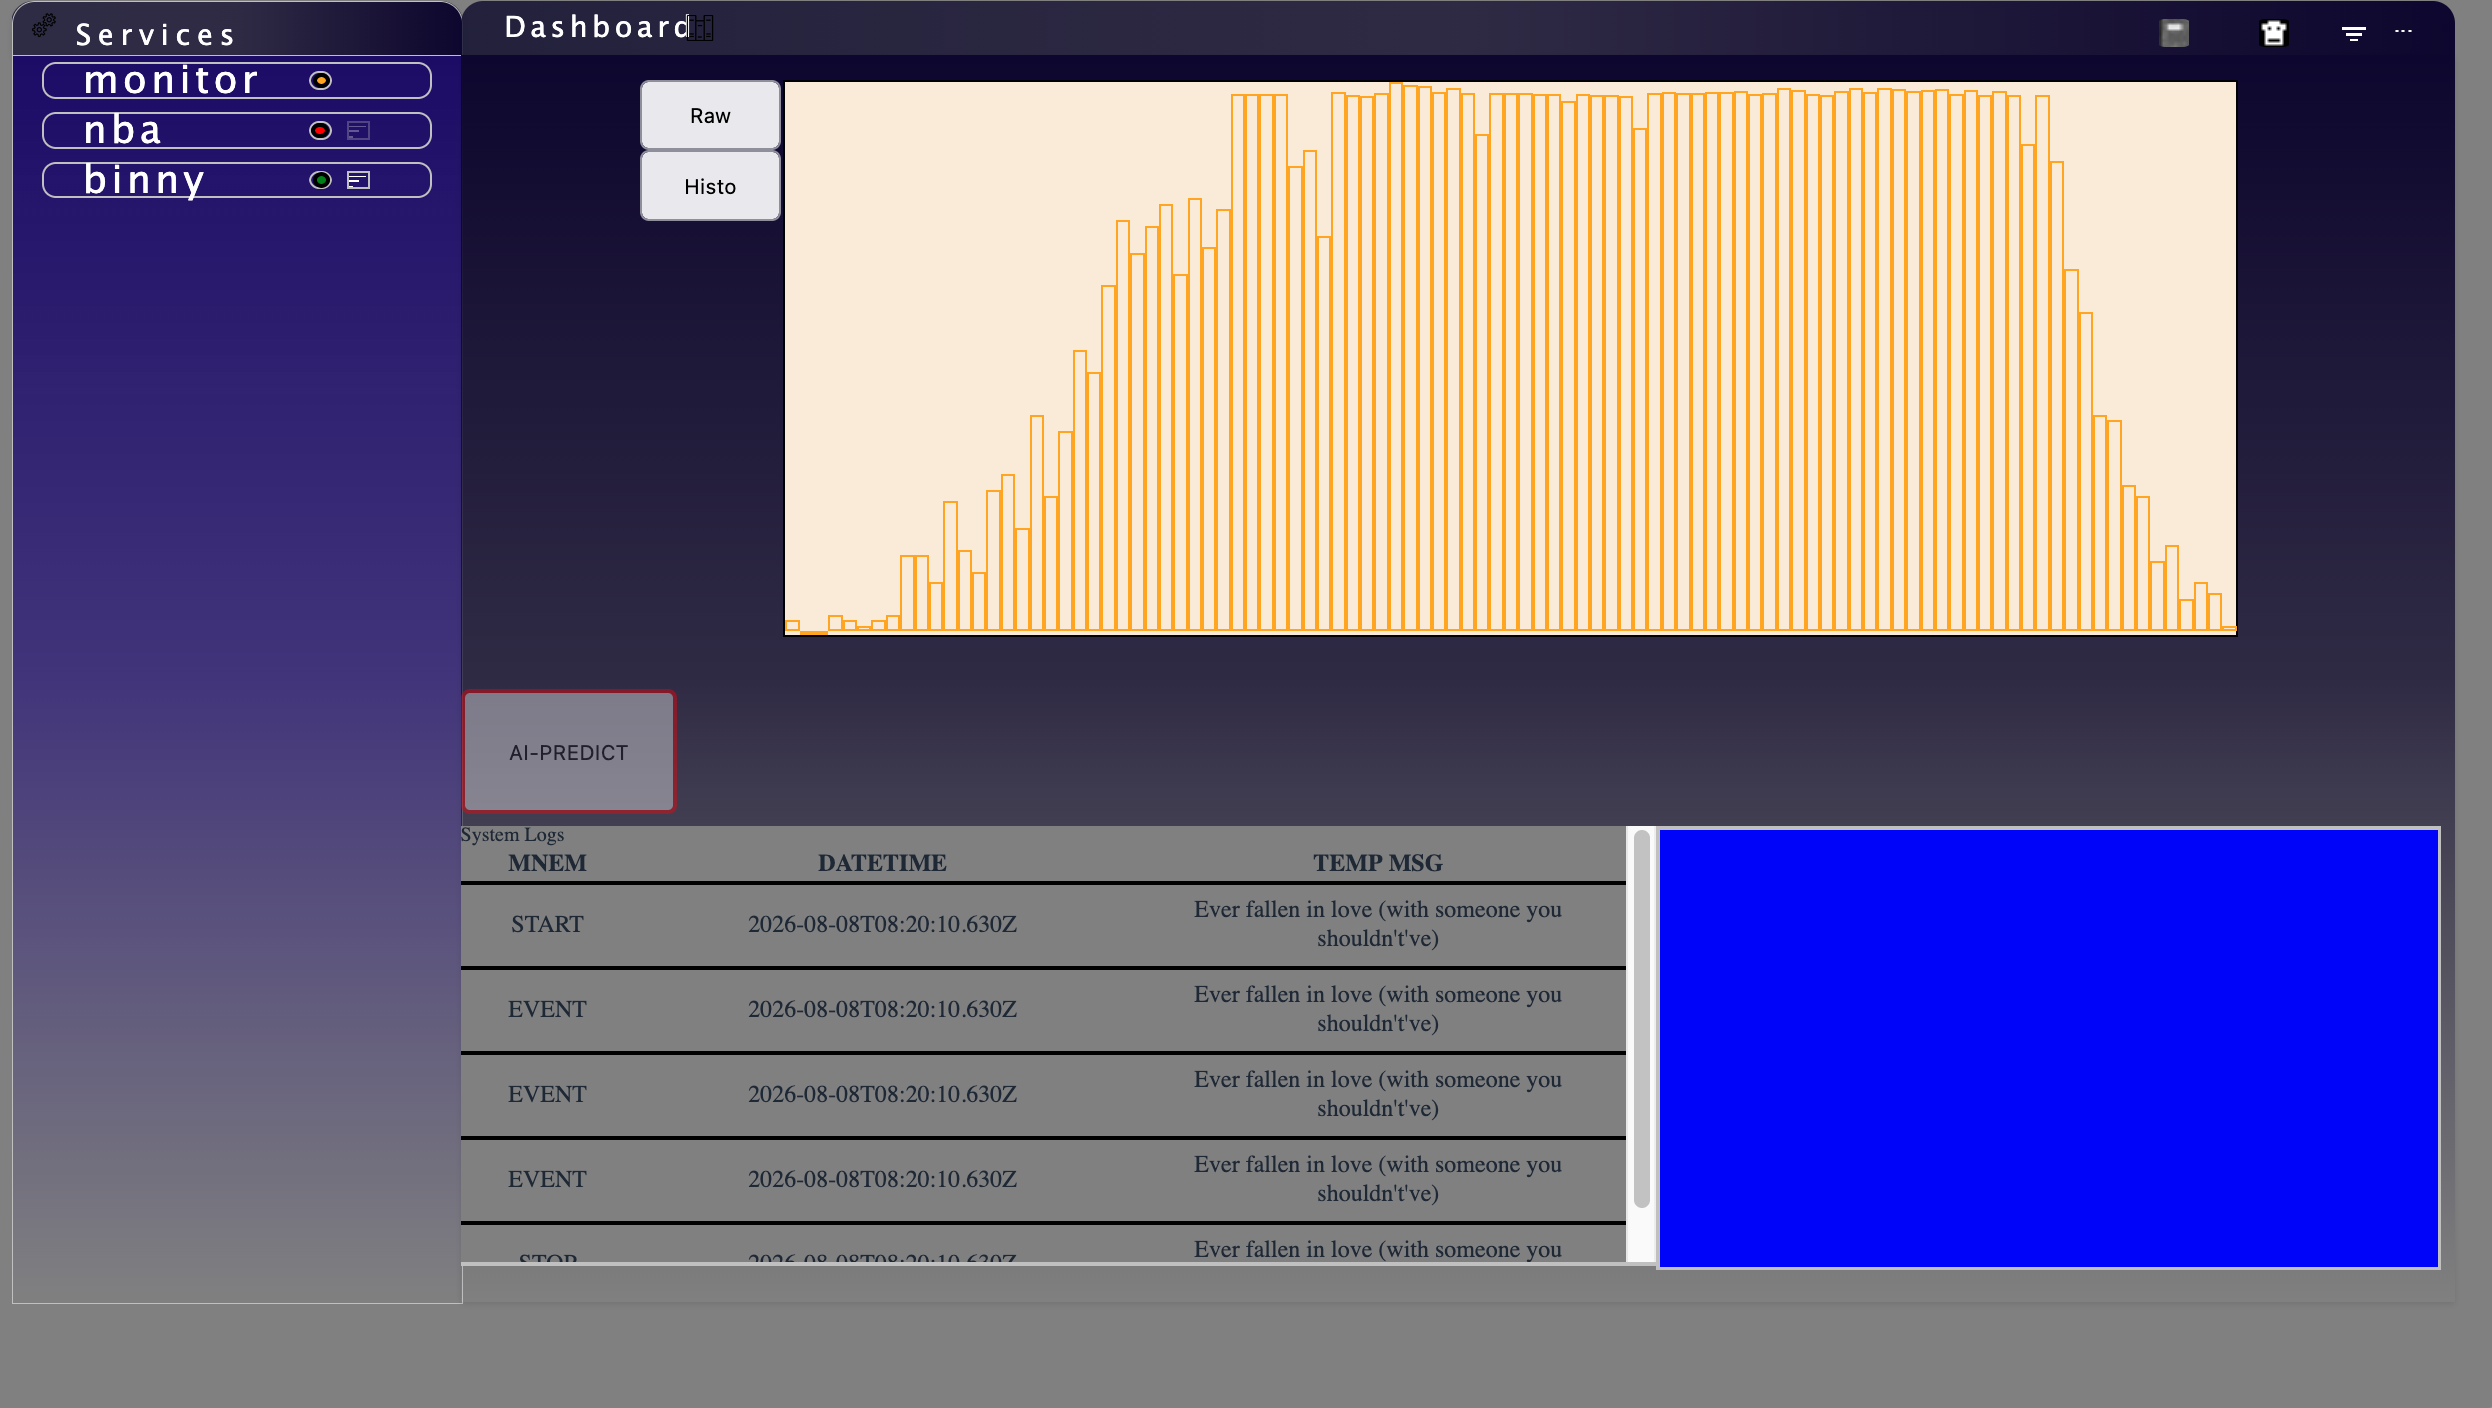
\includegraphics[width=1.0\textwidth, height=0.27\textheight]{image3}
            
            \caption{\textbf{GET }Binny Service - Histo}
        
            \label{fig:xyhisto}

        \end{figure}


        \begin{figure}[H]
            
            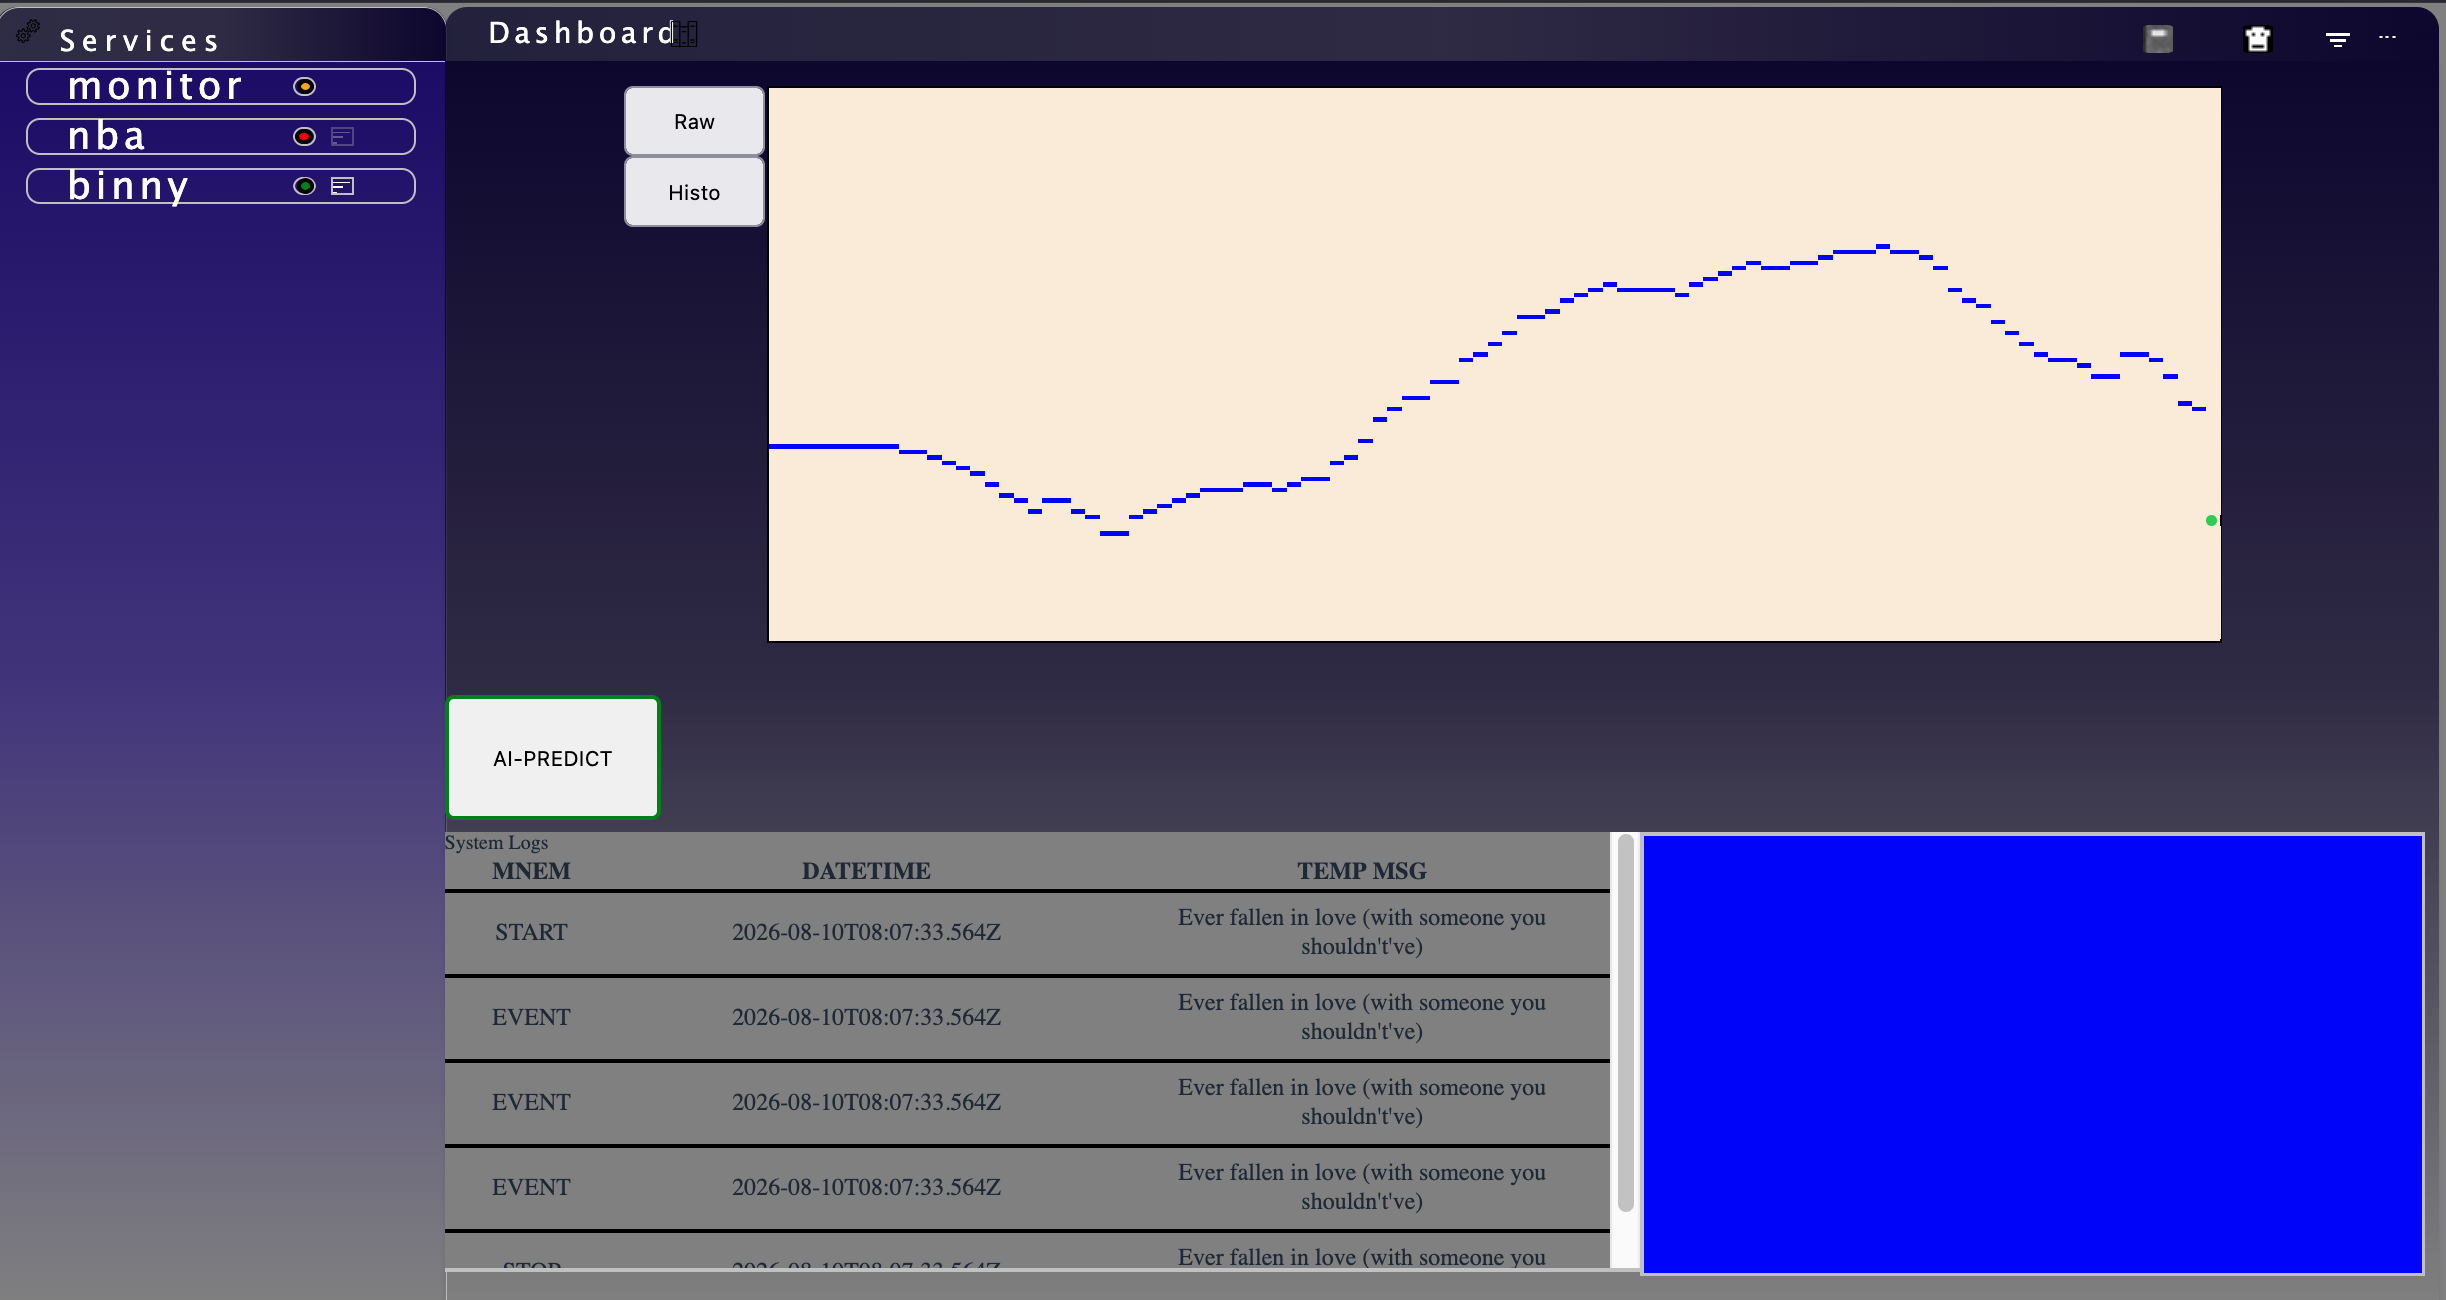
\includegraphics[width=1.0\textwidth, height=0.27\textheight]{image4}
            
            \caption{\textbf{GET } Model Prediction Service}
        
            \label{fig:forecast}

        \end{figure}

    
    \newpagex
    \noindent 
    \section{Load Temperature Train Data into DB}

    We used temperature data from Kaggle  \textit{\tiny\url{ https://www.kaggle.com/datasets/bhanupratapbiswas/weather-data} } to represent log data. The prediction model will be used predict potential future logs; this will be discussed in a future section.
    
    \noindent 
    \subsection{Loading data into database}
        
    \begin{itemize}
        \item Download WeatherData.csv aforementioned above and lowercase the filename.
        \item Move weatherdata.csv into nba\_app\textbackslash{}database\textbackslash{}pgfiles directory
        \item Create sql file (e.g. index2.sql) with schema matching the features labeled in WeatherData.csv
    
        \begin{verbatim}
CREATE TABLE  binny.temp (
    date_time text,
    temp real , 
    dew_point_temp real,
    humidity decimal, 
    wind_speed decimal,
    visibility decimal,
    weather text
    );
    \end{verbatim}
        \item Create script copyweather.sh in nba\_app\textbackslash{}database\textbackslash{}pgfiles \\ \smallskip 
        \textit{copyweather.sh}
        \begin{verbatim}
DB=sport_db
USER=htron
psql  -d "${DB}" --username "${USER}"  <<< "\copy binny.temp \
FROM '/root/work/WeatherData.csv' DELIMITER ',' CSV HEADER"
        \end{verbatim}

        \item Add the following commands to nba\_app\textbackslash{}database\textbackslash{}run.sh \\ \smallskip 
        \textit{run.sh}

        \begin{verbatim} 

DB=sport_db
USER=htron
docker exec "${CONTAINER_ID}" psql -d "${DB}"  --username "${USER}" -f /root/work/index2.sql

docker cp ./pgfiles/copyweather.sh \
<CONTAINER_ID\>:/root/work/copyweather.sh

docker cp ./pgfiles/weatherdata.csv \ 
<CONTAINER_ID\>:/root/work/weatherdata.csv

stdout=$(docker exec "${CONTAINER_ID}" \
./root/work/copyweather.sh & ) 
echo $stdout
        \end{verbatim} 
    \end{itemize}


    \newpagex
    \noindent 
    \section{View Database Table}
    Let's view the  weather table 
    \begin{itemize}
    \item Access PostgreSQL container (i.e. username=htron )  \smallskip
    \begin{verbatim} 
docker exec -it nba-pg psql -d sport\db --username htron
    \end{verbatim} 

    \item Verify binny table exist  \smallskip
    \begin{verbatim} 

sport\_db=> \dt binny.*

    List of tables
Schema | Name | Type  | Owner 
--------+------+-------+-------
binny  | temp | table | htron

 
sport_db=> select * from binny.temp;

    date_time     | temp  | dew_point_temp | humidity | wind_speed | visibility |  kpa   |                 weather                 
------------------+-------+----------------+----------+------------+------------+--------+-----------------------------------------
 1/1/2012 0:00    |  -1.8 |           -3.9 |       86 |          4 |          8 | 101.24 | Fog
 1/1/2012 1:00    |  -1.8 |           -3.7 |       87 |          4 |          8 | 101.24 | Fog
 1/1/2012 2:00    |  -1.8 |           -3.4 |       89 |          7 |          4 | 101.26 | Freezing Drizzle,Fog
 1/1/2012 3:00    |  -1.5 |           -3.2 |       88 |          6 |          4 | 101.27 | Freezing Drizzle,Fog
 1/1/2012 4:00    |  -1.5 |           -3.3 |       88 |          7 |        4.8 | 101.23 | Fog
 1/1/2012 5:00    |  -1.4 |           -3.3 |       87 |          9 |        6.4 | 101.27 | Fog
 1/1/2012 6:00    |  -1.5 |           -3.1 |       89 |          7 |        6.4 | 101.29 | Fog
 1/1/2012 7:00    |  -1.4 |           -3.6 |       85 |          7 |          8 | 101.26 | Fog
 1/1/2012 8:00    |  -1.4 |           -3.6 |       85 |          9 |          8 | 101.23 | Fog
 1/1/2012 9:00    |  -1.3 |           -3.1 |       88 |         15 |          4 |  101.2 | Fog
 1/1/2012 10:00   |    -1 |           -2.3 |       91 |          9 |        1.2 | 101.15 | Fog
 1/1/2012 11:00   |  -0.5 |           -2.1 |       89 |          7 |          4 | 100.98 | Fog
 1/1/2012 12:00   |  -0.2 |             -2 |       88 |          9 |        4.8 | 100.79 | Fog
 1/1/2012 13:00   |   0.2 |           -1.7 |       87 |         13 |        4.8 | 100.58 | Fog
 1/1/2012 14:00   |   0.8 |           -1.1 |       87 |         20 |        4.8 | 100.31 | Fog
 1/1/2012 15:00   |   1.8 |           -0.4 |       85 |         22 |        6.4 | 100.07 | Fog
 1/1/2012 16:00   |   2.6 |           -0.2 |       82 |         13 |       12.9 |  99.93 | Mostly Cloudy
 1/1/2012 17:00   |     3 |              0 |       81 |         13 |       16.1 |  99.81 | Cloudy
 1/1/2012 18:00   |   3.8 |              1 |       82 |         15 |       12.9 |  99.74 | Rain
 1/1/2012 19:00   |   3.1 |            1.3 |       88 |         15 |       12.9 |  99.68 | Rain
 1/1/2012 20:00   |   3.2 |            1.3 |       87 |         19 |         25 |   99.5 | Cloudy

        \end{verbatim} 
    \end{itemize}
    

    \newpagex
    \noindent 
    \section{Tensorflow Model Export}
    A tensorflow built sequence-to-vector network is exported into our Binny service. Our AI-Predict button infers the model. The following steps were used to create and load model.
    \begin{itemize}
        \item Create virtual environment using python 3.10  
        \item Install package housing command-line utility tensorflowjs\_converter : 
        \begin{verbatim} 
pip install --upgrade protobuf
pip install --upgrade tensorflowjs  
        \end{verbatim} 
        \item Train dataset (i.e. temperature in this case) using your preferred network of choice.   
        \item Networks   

        \begin{itemize}
            \item DNN Stateless Model 
            \begin{verbatim} 
s_model = tf.keras.models.Sequential()
s_model.add(keras.Input(shape=(N_SAMPLES,)))
s_model.add(keras.layers.Dense(N_SAMPLES, activation='selu'))
s_model.add(keras.layers.Dense(N_SAMPLES /2, activation='selu'))
s_model.add(keras.layers.Dense(N_SAMPLES / 3 + 1 , activation='selu'))
            \end{verbatim} 
        
        \item DNN Recurrent Network
            \begin{verbatim} 
input_ = tf.keras.layers.Input(shape=(N_SAMPLES, 1), batch_size = 32, dtype = tf.float32, name= "layer_in")
x = keras.layers.GRU(1, return_sequences=True, unroll=True, activation="selu", name="layer_gru1")(input_)
x = keras.layers.GRU(1, unroll=True, activation="selu", name="layer_gru2")(x)
output_ = keras.layers.Dense(1, name="layer_dense_out")(x)
s_model = keras.Model(inputs=input_, outputs=output_)
            \end{verbatim} 
        \end{itemize}

        \item Convert python keras model to Tensorflow.js   
            \begin{verbatim} 
tensorflowjs_converter --input_format=tf_saved_model --output_format=tfjs_graph_model $PWD/saved_model $PWD/web_model             
            \end{verbatim} 
        \item Export model  \smallskip 
            \small\textit{The exported model must use static shapes and not contain dynamic control flow operations(i.e.  while loops in graph model)}.
        \item Make server route to infer model    \smallskip 
        \item Validate ( Test event/inference)  \smallskip 
        
    \end{itemize} 
\end{document}


